\documentclass{article}

\usepackage{fancyhdr}
\usepackage{lastpage}
\usepackage{extramarks}
\usepackage[usenames,dvipsnames]{color}
\usepackage{graphicx}
\usepackage{listings}
\usepackage{courier}
\usepackage{lipsum}
\usepackage{fontspec}
\usepackage{xeCJK}
\setCJKmainfont{標楷體} 
\XeTeXlinebreaklocale "zh"
\XeTeXlinebreakskip = 0pt plus 1pt
\usepackage{indentfirst}
\usepackage[a4paper,margin=1.3in]{geometry}
\usepackage{graphicx}

\pagestyle{fancy}
\rhead{\hmwkClass \hmwkTitle}
\cfoot{}
\rfoot{Page\ \thepage\ of\ \protect\pageref{LastPage}}
\renewcommand\headrulewidth{0.4pt}
\renewcommand\footrulewidth{0.4pt}
\setlength\parindent{0pt} % Removes all indentation from paragraphs

\newcommand{\hmwkTitle}{Assignment 3}
\newcommand{\hmwkClass}{Information Security and Cryptography}
\newcommand{\hmwkClassInstructor}{教授:游家牧}
\newcommand{\hmwkAuthorName}{林家賢、黃川哲、黃晟慶、陳勇瑜、许萌}

\title{
\vspace{2in}
\textmd{\textbf{\hmwkClass\ \\  \hmwkTitle}}\\
\vspace{0.1in}\large{\textit{\hmwkClassInstructor}}\\
\vspace{0.1in}
網站:https://login.stufinite.faith
\vspace{2.9in}
}

\author{\textbf{\hmwkAuthorName}}
\date{}

\begin{document}

\maketitle

\newpage

\section{FHE}

\subsection{Install HElib}

\paragraph*{使用 Ubuntu 14.04 LTS}

\paragraph*{What we need?}
\begin{itemize}
\item GMP
\begin{itemize}
\item \verb|到 https://gmplib.org/#DOWNLOAD 選擇lz|
\item 解壓縮:tar --lzip -xvf gmp-6.1.2.tar.lz
\item cd gmp-6.1.2
\item 檢查需要的dependencies,產生Makefile:./configure
\end{itemize}
\centerline{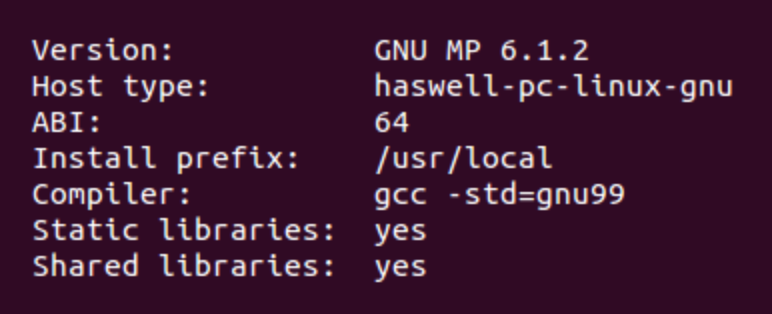
\includegraphics[width=0.80\textwidth]{make.png}}
\begin{itemize}
\item make
\begin{itemize}
\item 第一次報錯:缺m4
\begin{itemize}
\item sudo apt-get install m4
\end{itemize}
\end{itemize}
\begin{itemize}
\item 第二次報錯:/mpn/m4-ccas: Permission Denied
\begin{itemize}
\item chmod +x mpn/m4-ccas
\end{itemize}
\end{itemize}
\begin{itemize}
\item 第三次報錯:missing makeinfo
\begin{itemize}
\item sudo apt-get install texinfo
\end{itemize}
\end{itemize}
\item 不斷下載缺失的檔案直到沒有報錯後
\item sudo make install
\end{itemize}
\centerline{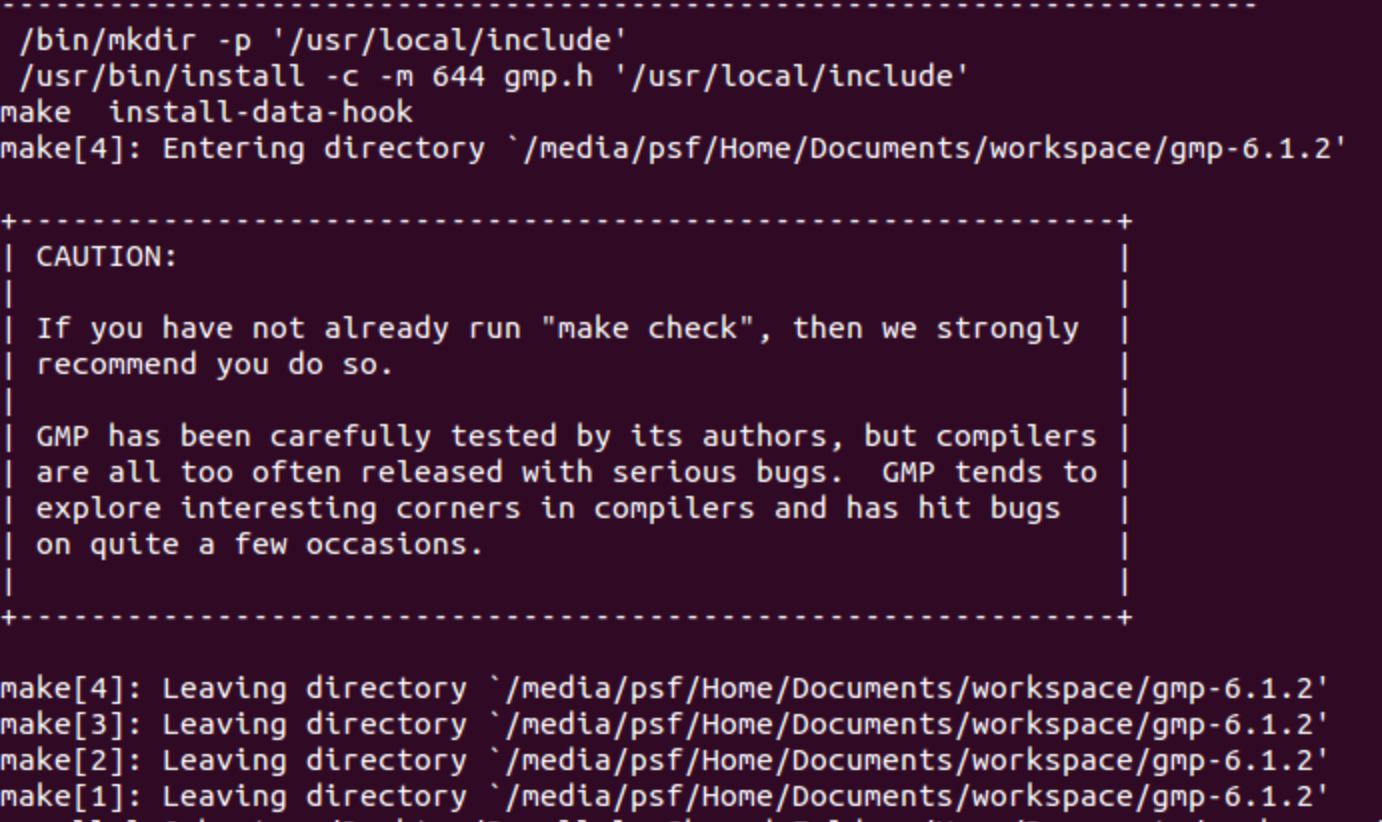
\includegraphics[width=1\textwidth]{install.png}}
\item NTL
\begin{itemize}
\item 到 http://www.shoup.net/ntl/download.html : 選擇10.3.0
\item 解壓縮
\item cd /ntl/10.3.0
\item \verb|./configure NTL_GMP_LIP=on|
\item make
\begin{itemize}
\item 報錯:g++ no found.
\begin{itemize}
\item sudo apt-get g++
\end{itemize}
\end{itemize}
\centerline{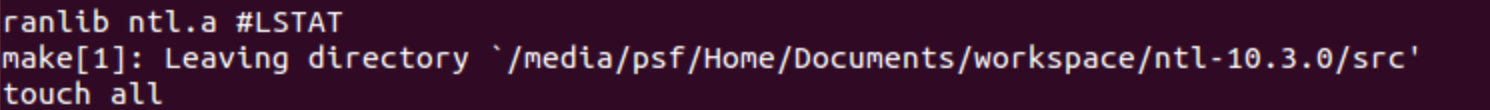
\includegraphics[width=1\textwidth]{getg++.png}}
\item sudo make install
\begin{itemize}
\item 最後會在 /usr/local/include 找到
\end{itemize}
\centerline{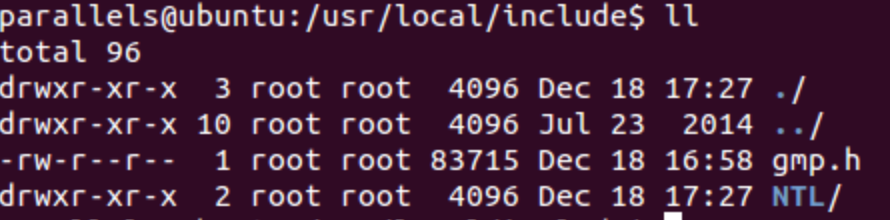
\includegraphics[width=0.80\textwidth]{NTL.png}}
\end{itemize}
\item 安裝HElib
\begin{itemize}
\item git clone https://github.com/shaih/HElib.git
\item make
\item make check
\end{itemize}
\centerline{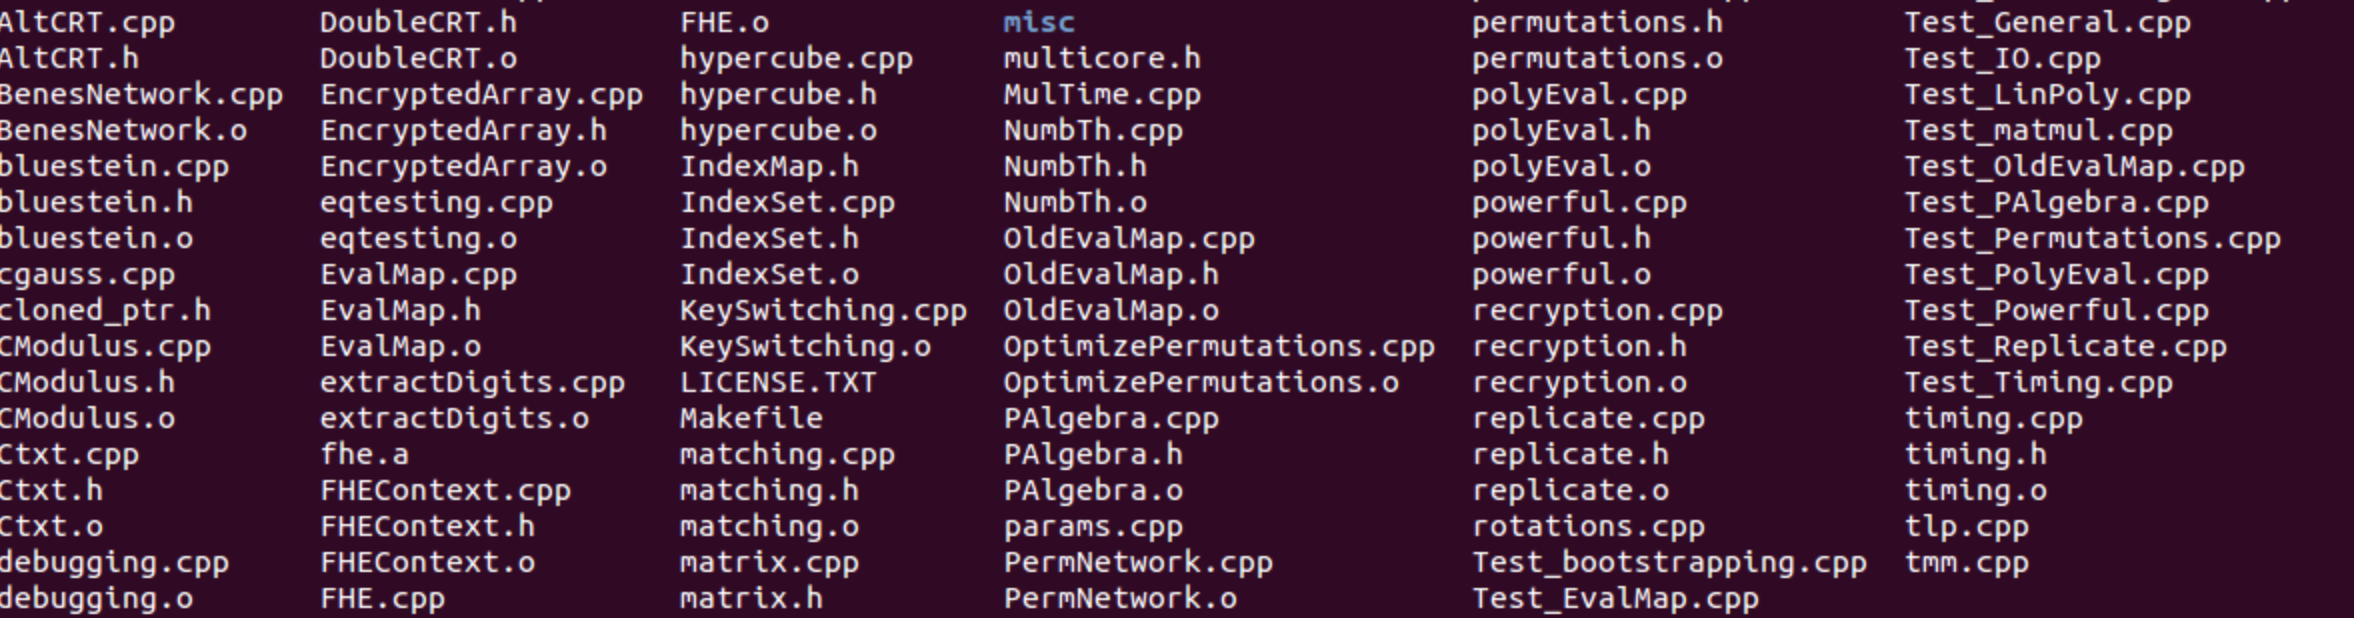
\includegraphics[width=1\textwidth]{HElib.png}}
\end{itemize}
 
 \subsection{HElib code}
 
\centerline{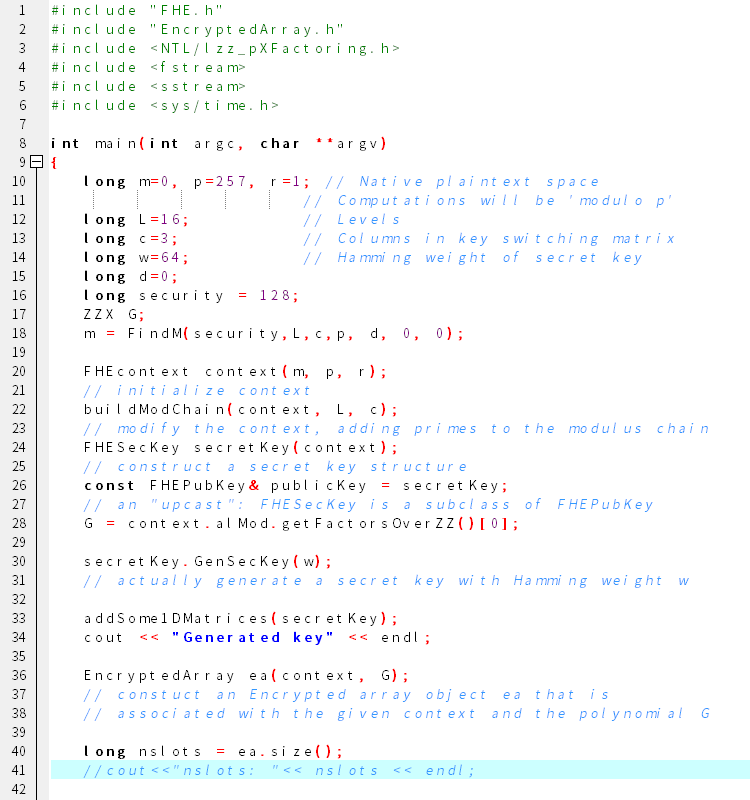
\includegraphics[width=1\textwidth]{HElibcode1.png}}
\begin{itemize}
\item Include some needed header.
\item We set some parameters for initialization, basically just copy and paste them.
\item "p" must be a prime number, we commonly hope it the larger the better.
\item We use these to create a "EncryptedArray" named "ea", and create "nslot" equal to ea.
\end{itemize}
\centerline{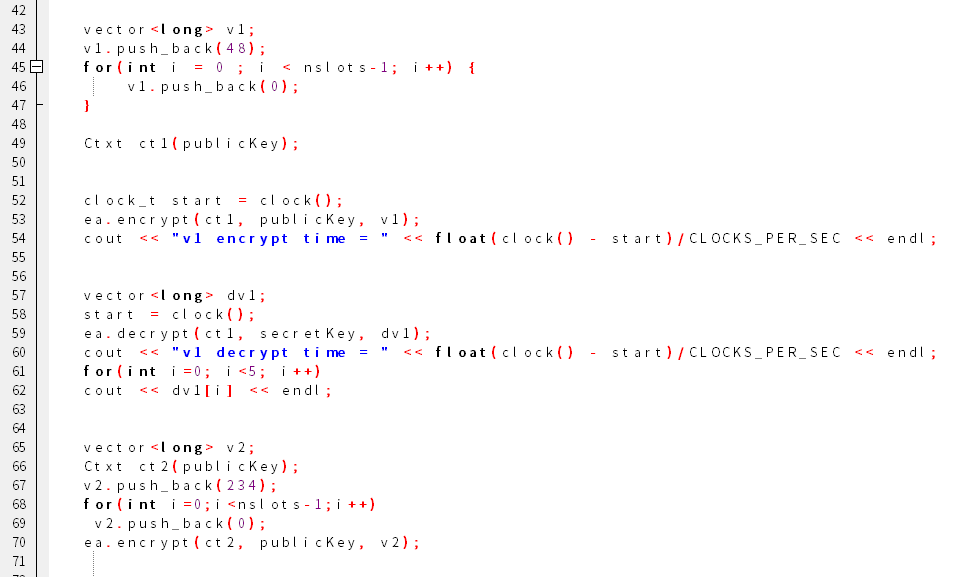
\includegraphics[width=1\textwidth]{HElibcode2.png}}
\begin{itemize}
\item "vector" is a data structure support by c++. Most of the time you can use it as a array.
\item "push\verb|_|back" can append something to a vector object. We set this vector as 48 and pad 0 until its length is equal to ea.
\item Create a "Ctxt" object to store encrypted v1, and measure time Consumption.
\item Create a "vector" dv1 to store decrypted ct1, and measure time Consumption.
\item Create another "vector" and encrypt it as "Ctxt" named ct2. 
\end{itemize}
\centerline{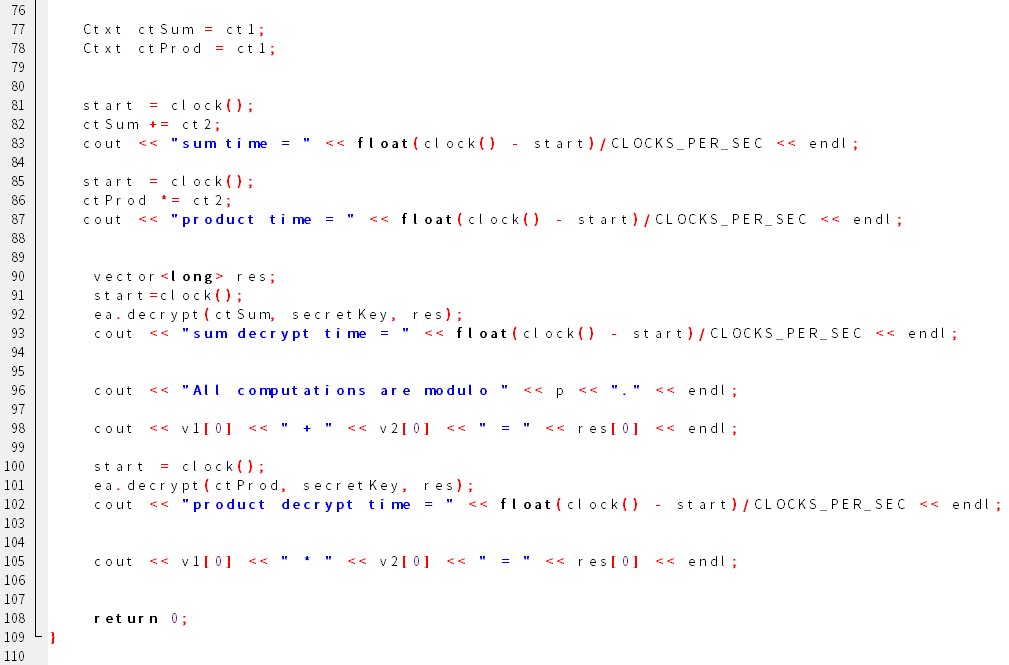
\includegraphics[width=1\textwidth]{HElibcode3.png}}
\begin{itemize}
\item Create two "Ctxt" named ctSum and CtProd.
\item Just add and multiply ct1 and ct2.
\item Then decrypt them.
\end{itemize}

\subsection{Time}
\centerline{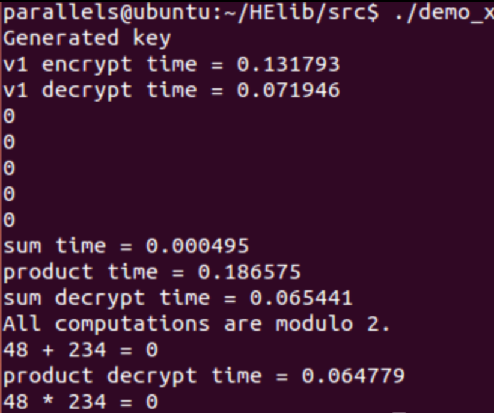
\includegraphics[width=0.6\textwidth]{HElibtime.png}}
 
 
 
 
 \section{PHE}
 
\subsection{Install Paillier}
 
\paragraph*{Our environment}
\begin{itemize}
\item Debian Jessie
\item  Python 2.7.9
\end{itemize}

\subparagraph{Install paillier from Github using pip}
\begin{itemize}
\item \verb|$ pip install -e git://github.com/mikeivanov/paillier.git#egg=paillier|
\end{itemize}

\subsection{Paillier code}

\centerline{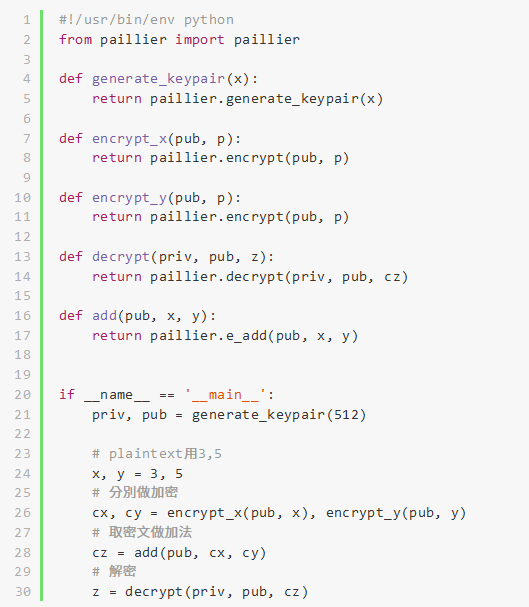
\includegraphics[width=1\textwidth]{pailliercode.png}}
\begin{itemize}
\item Paillier is much easier. We only need to import it, and use its function.
\item In our code, "generate keypair" parameter x is the length of key pairs; pub is public key; priv is private key; p is plaintext; cz is ciphertext which we want to decrypt; "add" parameter x and y are encrypted text.
\item So we just use these functions to measure time Consumption, but paillier doesn't support encrypted multiplication so we don't need to test it.
\end{itemize}

\subsection{Time}

\centerline{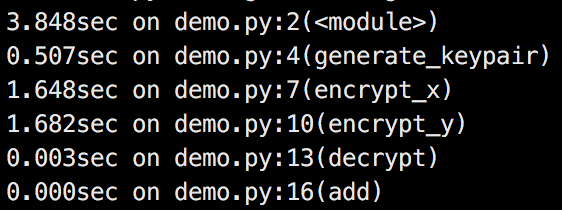
\includegraphics[width=0.70\textwidth]{pailliertime.png}}

\end{document}